\section{State of the Art}

The goal of PyTables is to enable the end user to manipulate
easily data \emph{tables} and \emph{array} objects in a 
hierarchical structure. The foundation of the underlying
hierarchical data organization is the HDF5 library \cite{TheHDFGroup2010}.

It should be noted that this package is not intended to serve as a
complete wrapper for the entire HDF5 API, but only to provide a
flexible, \emph{very pythonic} tool to deal with
(arbitrarily) large amounts of data (typically bigger than available
memory) in tables and arrays organized in a hierarchical and persistent
disk storage structure.

A table is defined as a collection of records whose values are
stored in \emph{fixed-length} fields. All records have the
same structure and all values in each field have the same \emph{data type}. 
The terms \emph{fixed-length} and strict data types may seem to be a strange requirement for
an interpreted language like Python, but they serve a useful function if
the goal is to save very large quantities of data (such as is generated
by many data acquisition systems, Internet services or scientific
applications, for example) in an efficient manner that reduces demand on
CPU time and I/O.

In order to emulate in Python records mapped to HDF5 C structs
PyTables implements a special class so as to easily define all its
fields and other properties. PyTables also provides a powerful interface
to mine data in tables. Records in tables are also known in the HDF5
naming scheme as \emph{compound} data types.

For example, you can define arbitrary tables in Python simply by
declaring a class with named fields and type information, such as in the
following example:

\vspace{2.5mm}
\begin{python}
class Particle(IsDescription):
    name      = StringCol(16)   # 16-character String
    idnumber  = Int64Col()      # signed 64-bit integer
    ADCcount  = UInt16Col()     # unsigned short integer
    TDCcount  = UInt8Col()      # unsigned byte
    grid_i    = Int32Col()      # integer
    grid_j    = Int32Col()      # integer

    # A sub-structure (nested data-type)
    class Properties(IsDescription):
        pressure = Float32Col(shape=(2,3)) # 2-D float array (single-precision)
        energy   = Float64Col(shape=(2,3,4)) # 3-D float array (double-precision)
\end{python}
\vspace{2.5mm}


You then pass this class to the table constructor, fill its rows
with your values, and save (arbitrarily large) collections of them to a
file for persistent storage. After that, the data can be retrieved and
post-processed quite easily with PyTables or even with another HDF5
application (in C, C++, Fortran, Java, Perl, and other languages which provide 
an interface to HDF5).

Other important entities in PyTables are
array objects, which are analogous to tables with
the difference that all of their components are homogeneous. They come
in different flavors, like \emph{generic} (they provide a
quick and fast way to deal with for numerical arrays),
\emph{enlargeable} (arrays can be extended along a single
dimension) and \emph{variable length} (each row in the
array can have a different number of elements).




\subsection{Main Features}

PyTables takes advantage of the object orientation and
introspection capabilities offered by Python, the powerful data
management features of HDF5, NumPy's flexibility, and Numexpr's
high-performance manipulation of large sets of objects organized in a
grid-like fashion to provide the following features.

\begin{itemize}
\item \textbf{Support for table entities:} Data sets may be tailored by
  adding or deleting records in tables. Large
  numbers of rows (up to 2\superscript{63} -- many more than will fit into memory)
  are supported as well.

\item \textbf{Multidimensional and nested table
  cells:} Columns can be declared to consist of values
  having any number of dimensions besides scalars, which is the only
  dimensionality allowed by the majority of relational databases.
  Nested columns that are made of other columns (of
  different types) may also be declared.

\item \textbf{Indexing support for columns of tables:}
  This feature, common in SQL, is very useful for large tables and which 
  must be quickly queried for values in columns satisfying some criteria.

\item \textbf{Support for numerical arrays:}
  NumPy \cite{Oliphant2007} arrays can be used as a useful 
  complement of tables to store homogeneous data.

\item \textbf{Enlargeable arrays:} New
  elements may be added to existing arrays on disk in any desired, single dimension.
  Moreover, access just a slice of a 
  dataset is granted by using the powerful extended slicing mechanism, without
  the need to load the complete dataset in memory.

\item \textbf{Variable length arrays:} The number of
  elements in these arrays can vary from row to row. This provides a
  lot of flexibility when dealing with complex data.

\item \textbf{Supports a hierarchical data model:}
  Allows the user to clearly structure all data. PyTables builds up
  an \emph{object tree} in memory that replicates the
  underlying file data structure. Access to objects in the file is
  achieved by walking through and manipulating this object tree.
  Besides, this object tree is built in a lazy way, for efficiency
  purposes.

\item \textbf{User defined metadata:} Besides
  supporting system metadata (like the number of rows of a table,
  shape, flavor, etc.) the user may specify arbitrary metadata (as
  for example, room temperature, or protocol for IP traffic that was
  collected) that complement the meaning of actual data.

\item \textbf{Ability to read/modify generic HDF5
  files:} PyTables can access a wide range of objects in
  generic HDF5 files, like compound type datasets (that can be
  mapped to Table objects), homogeneous datasets
  (that can be mapped to Array objects) or
  variable length record datasets (that can be mapped to
  VLArray objects). Besides, if a dataset is not
  supported, it will be mapped to a special
  UnImplemented class,
  that will let the user see that the data is there, although it
  will be unreachable (the user is able to access the
  attributes and some metadata in the dataset). In practice, PyTables
  is capable of accessing and modifying the overwhelming majority of
  HDF5 files.

\item \textbf{Data compression:} Supports data
  compression (using the Zlib, LZO, bzip2
  and Blosc compression libraries) out of the
  box. This is important for repetitive data patterns and
  for searching over such data in an optimized way. This 
  reduces the time spent analyzing data due to organizational 
    overhead.

\item \textbf{High performance I/O:} On modern systems
  storing large amounts of data, tables and array objects can be
  read and written at a speed only limited by the performance of the
  underlying I/O subsystem. Moreover, if the data is compressible,
  even this I/O-bound limitation is surmountable.

\item \textbf{Support of files bigger than 2 GB:}
  PyTables automatically inherits this capability from the
  underlying HDF5 library (assuming your platform supports the C
  long long integer, or, on Windows, \_\_int64).

\item \textbf{Architecture-independent:} PyTables has
  been carefully coded (as HDF5 itself) with
  little-endian/big-endian byte ordering issues in mind. Thus, a
  file written on a big-endian machine (like a Sparc or MIPS) may be
  read on another little-endian machine (like an Intel or Alpha)
  without problems. In addition, it has been tested successfully
  with both 32 \& 64 bit platforms using code generated with a variety 
  of compilers.

\end{itemize}


\subsection{The Object Tree}

The hierarchical model of the underlying HDF5 library allows
PyTables to manage tables and arrays in a tree-like structure. In
order to achieve this, an object tree entity is
dynamically created imitating the HDF5 structure
on disk. The HDF5 objects are read by walking through this object
tree. What kind of data is kept in the object may be discovered 
by examining the \emph{metadata} nodes.

The different nodes in the object tree are instances of PyTables
classes. There are several types of classes, but the most important
ones are the Node, Group and
Leaf classes. All nodes in a PyTables tree are
instances of the Node class. The
Group and Leaf classes are
descendants of Node. Group
instances (referred to as \emph{groups} from now on) are
a grouping structure containing instances of zero or more groups or
leaves, together with supplementary metadata. Leaf
instances (referred to as \emph{leaves}) are containers
for actual data and can not contain further groups or leaves. The
Table, Array,
CArray, EArray,
VLArray and UnImplemented
classes are descendants of Leaf, and inherit all
its properties.

Working with groups and leaves is similar in many ways to
working with directories and files on a Unix file system, i.e. a node
(file or directory) is always a \emph{child} of one and
only one group (directory), its \emph{parent group}.
Inside of that group, the node is accessed by its
\emph{name}. As is the case with Unix directories and
files, objects in the object tree are often referenced by giving their
full (absolute) path names. In PyTables this full path can be
specified either as string (such as
\texttt{/subgroup2/table3}, using \texttt{/} as
a parent/child separator) or as a complete object path written in a
format known as the \emph{natural name} schema (such as
\texttt{file.root.subgroup2.table3}).

Support for \emph{natural naming} is a key aspect
of PyTables. It means that the names of instance variables of the node
objects are the same as the names of its children \cite{Mertz2000}. 
This is very Pythonic and intuitive in many cases. 

Note that not all the data present in a file
is loaded into the object tree. The metadata
(i.e. special data that describes the structure of the actual data) is
loaded only when the user accesses it. Moreover,
the actual data is not read until it is requested (by calling a method
on a particular node). Using the object tree (the metadata)
information may be retrieves about the objects on disk.  For tables 
this includes names, titles, column names, data types in columns, and the numbers of rows.
For the case of arrays their shapes, typecodes, etc may be retrieved. 
The tree may also be searched through for specific kinds of data then read in and processed.
Therefore PyTables as a tool that
applies the same introspection capabilities of Python objects to large
amounts of data in persistent storage.  This is capability that is not
present in the underlying HDF5 routines.

Furthermore, PyTables sports a \emph{metadata
cache system} that loads nodes \emph{lazily}
(i.e. on-demand), and unloads nodes that have not been used for some
time (following a \emph{Least Recently Used} schema). It
is important to stress that the nodes enter the cache after they
have been unreferenced (via Python reference counting),
and that they can be revived (by referencing them again) directly from
the cache without performing the de-serialization process from
disk. This feature allows dealing with files with large hierarchies
very quickly and with low memory consumption, while retaining all the
powerful browsing capabilities of the previous implementation of the
object tree. See \cite{Alted2005} for
more facts about the advantages introduced by this new metadata cache
system.

To better understand the dynamic nature of this object tree
entity, start with a sample PyTables script to create an HDF5
file:

\vspace{2.5mm}
\begin{python}
from tables import *

class Particle(IsDescription):
    identity = StringCol(itemsize=22, dflt=" ", pos=0)  # character string
    idnumber = Int16Col(dflt=1, pos = 1)  # short integer
    speed    = Float32Col(dflt=1, pos = 1)  # single-precision

# Open a file in "w"rite mode
fileh = openFile("objecttree.h5", mode = "w")

# Get the HDF5 root group
root = fileh.root

# Create the groups
group1 = fileh.createGroup(root, "group1")
group2 = fileh.createGroup(root, "group2")

# Now, create an array in root group
array1 = fileh.createArray(root, "array1", ["string", "array"], "String array")

# Create 2 new tables in group1
table1 = fileh.createTable(group1, "table1", Particle)
table2 = fileh.createTable("/group2", "table2", Particle)

# Create the last table in group2
array2 = fileh.createArray("/group1", "array2", [1,2,3,4])

# Now, fill the tables
for table in (table1, table2):
    # Get the record object associated with the table:
    row = table.row

    # Fill the table with 10 records
    for i in xrange(10):
        # First, assign the values to the Particle record
        row['identity']  = 'This is particle: %2d' % (i)
        row['idnumber'] = i
        row['speed']  = i * 2.

        # This injects the Record values
        row.append()

    # Flush the table buffers
    table.flush()

# Finally, close the file (this also will flush all the remaining buffers!)
fileh.close()
\end{python}
\vspace{2.5mm}

This small program creates a simple HDF5 file called
\texttt{objecttree.h5} with the structure that appears in
Figure \ref{objecttree-h5}.
When the file is created, the metadata in the object tree is updated
in memory while the actual data is saved to disk. When you close the
file the object tree is no longer available. However, when you reopen
this file the object tree will be reconstructed in memory from the
metadata on disk (this is done in a lazy way, in order to load only
the objects that are required by the user), allowing the user to work with
it in exactly the same way as when the user originally created it.

Figure \ref{objecttree}, is an example of the object tree created when the above
\texttt{objecttree.h5} file is read in.  In fact, such an object
tree is always created when reading any supported generic HDF5 file.
This demonstrates the relationships of in-memory PyTables objects.

\begin{figure}
\begin{center}
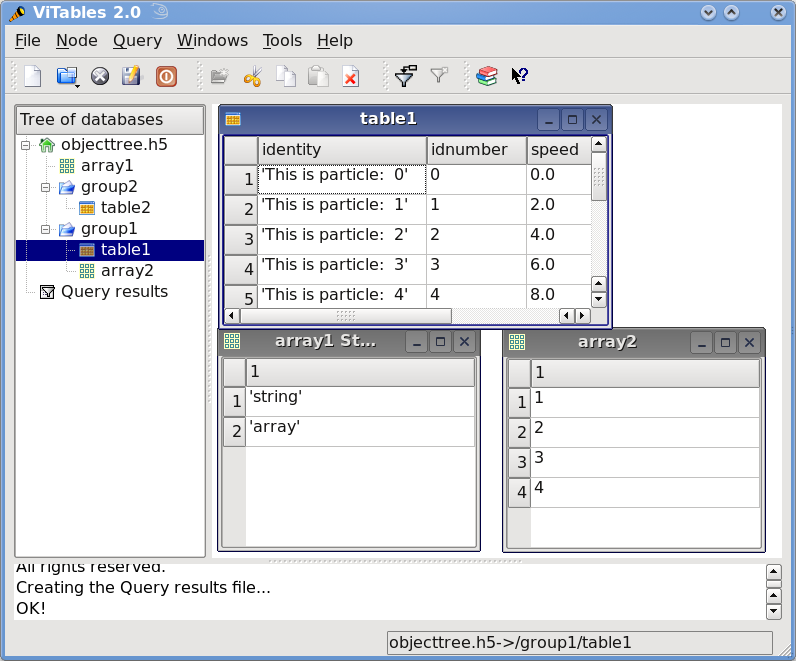
\includegraphics[scale=0.75]{figures/objecttree-h5.png}
\caption{An HDF5 example with 2 subgroups, 2 tables and 1 array.}
\label{objecttree-h5}
\end{center}
\end{figure}

\begin{figure}
\begin{center}
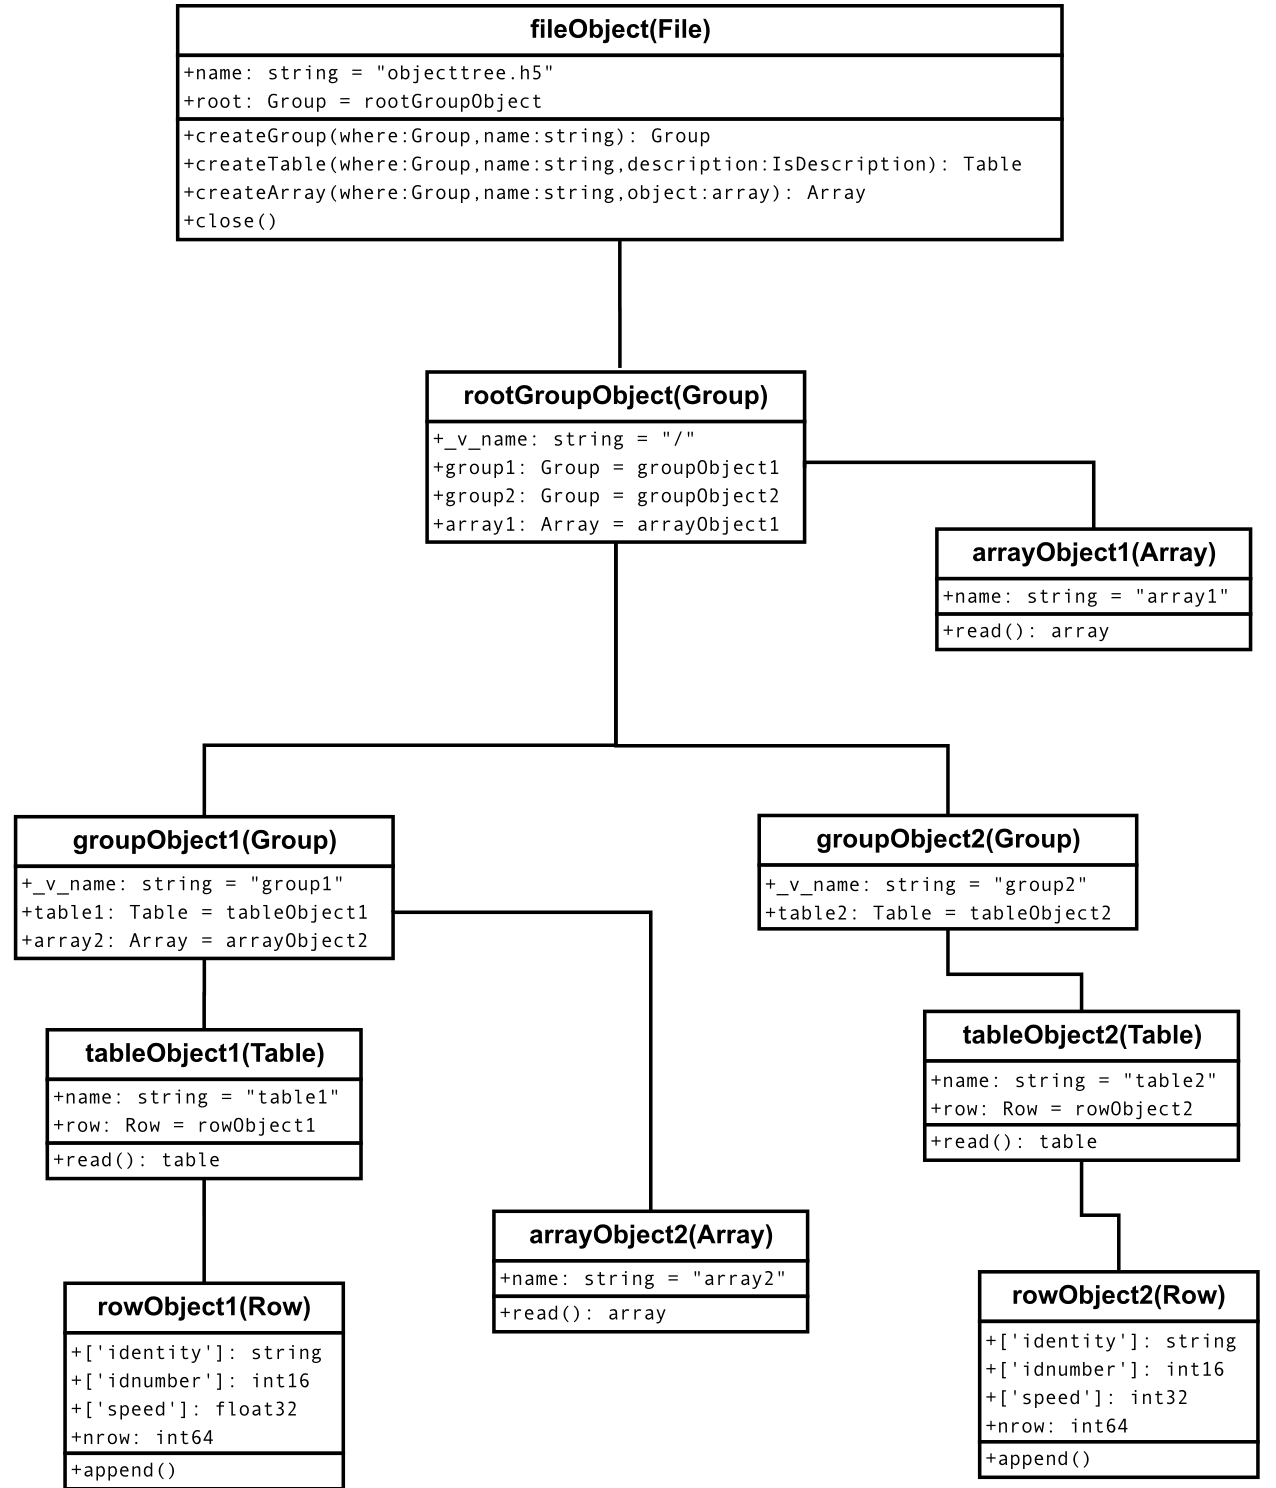
\includegraphics[scale=0.4]{figures/objecttree.png}
\caption{A PyTables object tree example.}
\label{objecttree}
\end{center}
\end{figure}
